%%%%%%%%%%%%%%%%%%%%%%%%%%%%%%%%%%%%%%%%%%%%%%%%%%%%%%%%%%%%%%%%%%%%%%%%%%%
%%%%%%%%%%%%%%%%%%%%%%%%%%%%%%%%%%%%%%%%%%%%%%%%%%%%%%%%%%%%%%%%%%%%%%%%%%%
%%
%% The basic tex file for the header of all the lectures. 
%%

\documentclass{beamer}
\usetheme[hideallsubsections]{Berkeley}

\usepackage{color}
\usepackage{amsfonts}

\definecolor{myblue}{rgb}{0.25, 0, 0.75}
\definecolor{mygold}{rgb}{1,0.8,0.2}
\definecolor{gray}{rgb}{0.5, 0.5, 0.5}
\definecolor{lucia}{rgb}{0.8,0.4,0.7} 

\newcommand{\myurl}[1]{\href{http://#1}{\textcolor{gray}{\texttt{#1}}}}
\newcommand{\myem}[1]{\structure{#1}}
\newcommand{\RPack}[1]{\textcolor{gray}{\textsf{#1}}}
\newcommand{\pl}[1]{\texttt{#1}}
\newcommand{\Rcode}[1]{\texttt{#1}}
\newcommand{\Rfunction}[1]{\href{http://www.statmethods.net/search/index.asp?QU=#1&search=Search&Action=Search}{\textcolor{orange}{\textsf{#1}}}}
\newcommand{\myurlshort}[2]{\href{http://#1}{\textcolor{gray}{\textsf{#2}}}}
\newcommand{\RClass}[1]{\textcolor{mygold}{\textsf{#1}}}
\newcommand{\BIOCfunction}[1]{\textcolor{orange}{#1}}

\setbeamercolor{example text}{fg=lucia}
\setbeamertemplate{sections/subsections in toc}[ball unumbered]
\setbeamertemplate{frametitle continuation}[from second][]
\setbeamertemplate{itemize subitem}[triangle]
\setbeamertemplate{footline}[page number]
\setbeamertemplate{caption}[numbered]

\renewcommand{\footnotesize}{\fontsize{6.10}{12}\selectfont}

\def\argmax{\operatornamewithlimits{arg\,max}}
\def\argmin{\operatornamewithlimits{arg\,min}}


%%%%%%%%%%%%%%%%%%%%%%%%%%%%%%%%%%%%%%%%%%%%%%%%%%%%%%%%%%%%%%%%%%%%%%%%%%%
\title{R / Bioconductor: Curso Intensivo}

\author[]{\myem{Leonardo Collado Torres}\\
  Licenciatura en Ciencias Gen�micas, UNAM\\
  \myurl{www.lcg.unam.mx/\string~lcollado/index.php}\\
}

\date{
  Cuernavaca, M�xico\\
  Oct-Nov, 2008
}






\usepackage{Sweave}
\begin{document}

%%% set up some options for Sweave and R %%%

%%%%%%%%%%%%%%%%%%%%%%%%%%%%%%%%%%%%%%%%%%%%%%%%%%%%%%%%%%%%%%%%%%%%%%%%%%%
%%%%%%%%%%%%%%%%%%%%%%%%%%%%%%%%%%%%%%%%%%%%%%%%%%%%%%%%%%%%%%%%%%%%%%%%%%%
\begin{frame}[allowframebreaks]
  \titlepage
\end{frame}

\begin{frame}[allowframebreaks]
  \frametitle{N�meros al azar}
  \tableofcontents
\end{frame}

%%%%%%%%%%%%%%%%%%%%%%%%%%%%%%%%%%%%%%%%%%%%%%%%%%%%%%%%%%%%%%%%%%%%%%%%%%%
\section{Conceptos}

\begin{frame}[allowframebreaks]
  \frametitle{Objetivos}
  \begin{itemize}
    \item Hoy vamos a aprender como sacar n�meros al azar y otros conceptos de estad�stica.
  \end{itemize}
\end{frame}

\begin{frame}[allowframebreaks]
  \frametitle{Funci�n de densidad}
  \begin{itemize}
    \item La funci�n de densidad de probabilidad nos dice como se distribuyen las probabilidades de un evento o suceso dado.
	\item En s�, es una integral y como la saben el �rea total bajo la curva de dicha funci�n es igual a 1.
	\end{itemize}
\end{frame}


\begin{frame}[allowframebreaks]
  \frametitle{Distribuci�n de probabilidad}
  \begin{itemize}
    \item Tambi�n conocida como \emph{distribuci�n de probabilidad acumulada} nos dice cu�l es la probabilidad de que $X$ sea menor o igual al valor que tengamos.
	\item Dicho de otra forma, $F_{X}(x) = P(X \leq x)$ donde $X$ es una variable aleatoria y su funci�n de distribuci�n es $F_{X}(x)$
  \end{itemize}
\end{frame}

\begin{frame}[allowframebreaks]
  \frametitle{Funci�n de cuantiles}
  \begin{itemize}
    \item Esta funci�n es la inversa $F^-1$ de la funci�n de distribuci�n acumulada. 
	\item Toma como valores de entrada probabilidades y nos regresa el valor debajo el cual n�meros obtenidos al azar con dicha distribuci�n caer�an el $p * 100$ porciento de las veces.
	\item Osea, $Pr(X \leq x) = p$
  \end{itemize}
\end{frame}

%%%%%%%%%%%%%%%%%%%%%%%%%%%%%%%%%%%%%%%%%%%%%%%%%%%%%%%%%%%%%%%%%%%%%%%%%%%
\section{Ahora en \pl{R}}

\begin{frame}[allowframebreaks, fragile]
  \frametitle{Unif}
  \begin{itemize}
  \item Ya con los conceptos anteriores\footnote{Si tienen dudas les recomendio Wikipedia en ingl�s} podemos pasar a R.
\begin{Schunk}
\begin{Sinput}
> `?`(runif)
\end{Sinput}
\end{Schunk}
  \item Ya deben conocer a \BIOCfunction{runif} pues la hemos usado algunas veces. Ahora ponganle un poco m�s de atenci�n.
  \end{itemize}
\end{frame}

\begin{frame}[allowframebreaks]
  \frametitle{Las 4 funciones}
  \begin{itemize}  
  \item Como ven, hay 4 usos con \BIOCfunction{unif}.
  \begin{enumerate}
    \item \pl{dunif} para usar la funci�n de densidad uniforme.
	\item \pl{punif} para la funci�n de prob. acumulada uniforme.
	\item \pl{qunif} para la funci�n de cuantiles uniforme.
	\item \pl{runif} para obtener n�meros al azar con una distribuci�n uniforme.
  \end{enumerate}
  \item \textquestiondown Por qu� $punif(u) = u$ y $dunif(u) = 1$ siendo $u$ veinte valores obtenidos con \pl{runif}?
  \end{itemize}
\end{frame}

\begin{frame}[allowframebreaks, fragile]
  \frametitle{Algo raro..}
  \begin{itemize}
  \item Ahora quiero que corran el siguiente comando\footnote{Si lo pon�a en la presentaci�n se hacia bastante grande :P}.
  \item \textquestiondown Qu� encuentran de raro? \alert{TIP} Usen \BIOCfunction{ylim} y/o \BIOCfunction{xlim}.
\begin{Schunk}
\begin{Sinput}
> plot(runif(10000))
\end{Sinput}
\end{Schunk}
  \end{itemize}
\end{frame}

\begin{frame}[allowframebreaks, fragile]
  \frametitle{Algo raro.. 2}
  \begin{itemize}
  \item Ahora prueben este c�digo. \textquestiondown Es lo que esperamos o hay algo raro?
\begin{Schunk}
\begin{Sinput}
> plot(runif(1000), rnorm(1000))
\end{Sinput}
\end{Schunk}
  \end{itemize}
\end{frame}

\begin{frame}[fragile]
  \frametitle{Graf. del 2}
  \begin{figure}[htbp] 
  \begin{centering}   
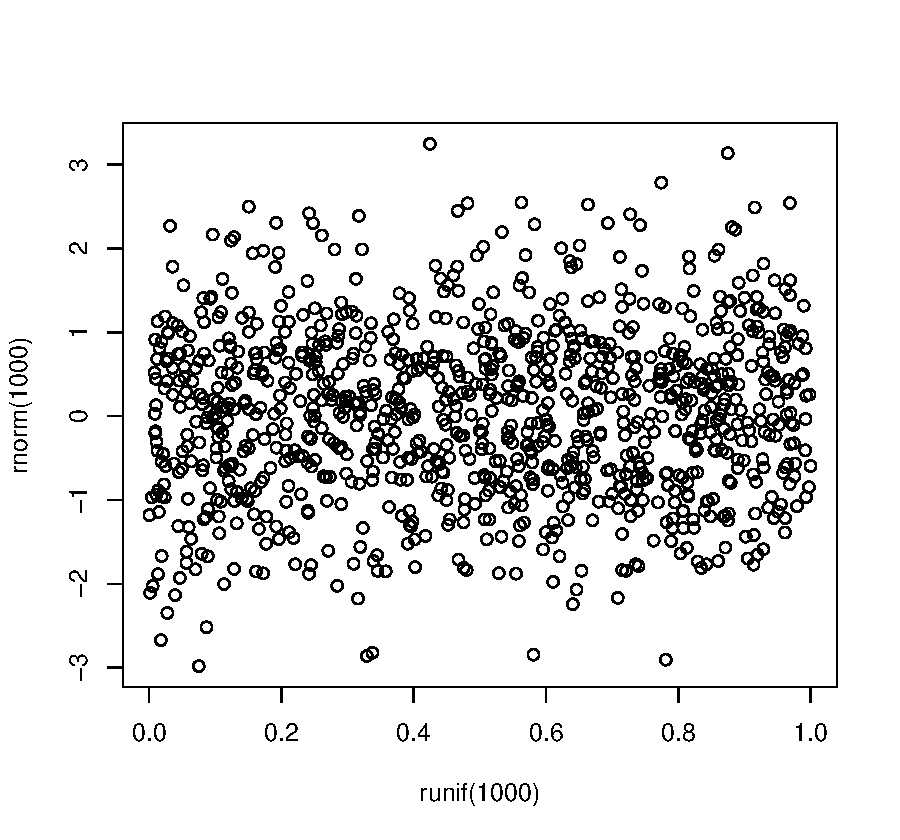
\includegraphics{plots/random-005}
  \end{centering} 
  \end{figure}
\end{frame}

%%%%%%%%%%%%%%%%%%%%%%%%%%%%%%%%%%%%%%%%%%%%%%%%%%%%%%%%%%%%%%%%%%%%%%%%%%%
\section{Un nuevo tipo de gr�fica}

\begin{frame}[allowframebreaks]
  \frametitle{Ja!}
  \begin{itemize}
  \item \textquestiondown No creen que es muy ineficiente esta forma de comparar distribuciones? Bueno, usemos algo mejor.
  \end{itemize}
\end{frame}

\begin{frame}[allowframebreaks]
  \frametitle{\BIOCfunction{boxplot}}
  \begin{itemize}
  \item Una gr�fica muy usada el \BIOCfunction{boxplot} que en s� utiliza la informaci�n del \Rcode{summary}. Con este tipo de gr�fica es f�cil visualizar:
  \begin{itemize}
    \item Los cuartiles 1, 2 y 3. \alert{Nota:} el segundo cuartil corresponde a la mediana.
    \item Te pone l�mites m�ximo y m�nimo usando el cuartil 1 - 1.5 veces el IQR\footnote{o rango intercuartilico por sus siglas en ingl�s}, el cuartil 3 + 1.5 veces IQR
	\item Los valores extremos. Estos aparecen como bolitas hasta arriba y/o abajo de los l�mites.
  \end{itemize}
  \item A continuaci�n les muestro un ejemplo:
  \end{itemize}
\end{frame}

\begin{frame}[fragile]
  \frametitle{Un ejemplo}
  \begin{figure}[htbp]
  \begin{centering}
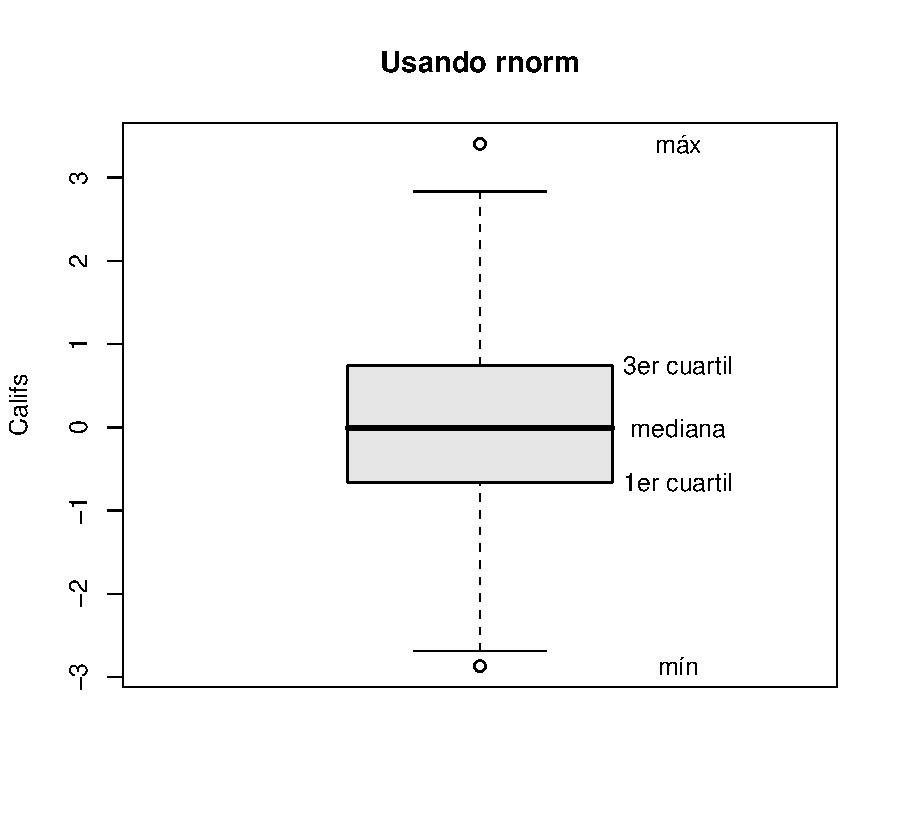
\includegraphics{plots/random-006}
  \end{centering}
  \end{figure}
\end{frame}

\begin{frame}[allowframebreaks, fragile]
  \frametitle{Terminando}
  \begin{itemize}
  \item Ya para terminar, ahora s� comparemos varias distribuciones:
\begin{Schunk}
\begin{Sinput}
> boxplot(runif(100), rnorm(100), 
+     rchisq(100, 1))
\end{Sinput}
\end{Schunk}
  \end{itemize}
\end{frame}  

\begin{frame}[fragile]
  \frametitle{\textquestiondown Se ve as�?}
  \begin{figure}[htbp] 
  \begin{centering}   
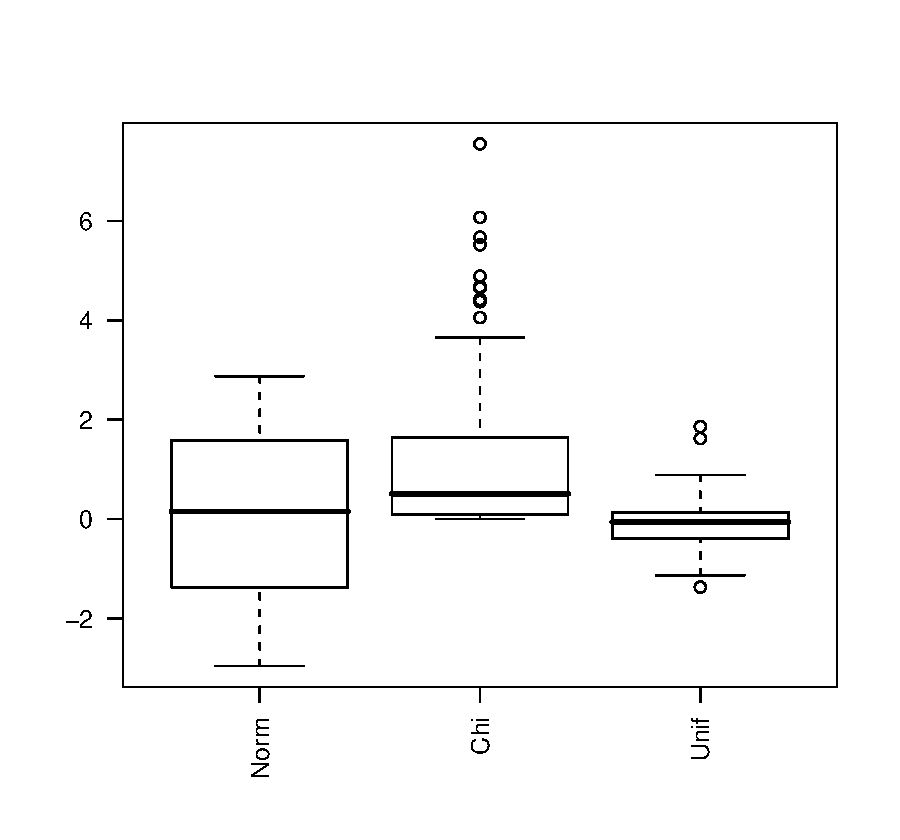
\includegraphics{plots/random-008}
  \end{centering} 
  \end{figure}
\end{frame}

\begin{frame}[fragile]
  \frametitle{\textquestiondown O as�?}
  \begin{figure}[htbp] 
  \begin{centering}   
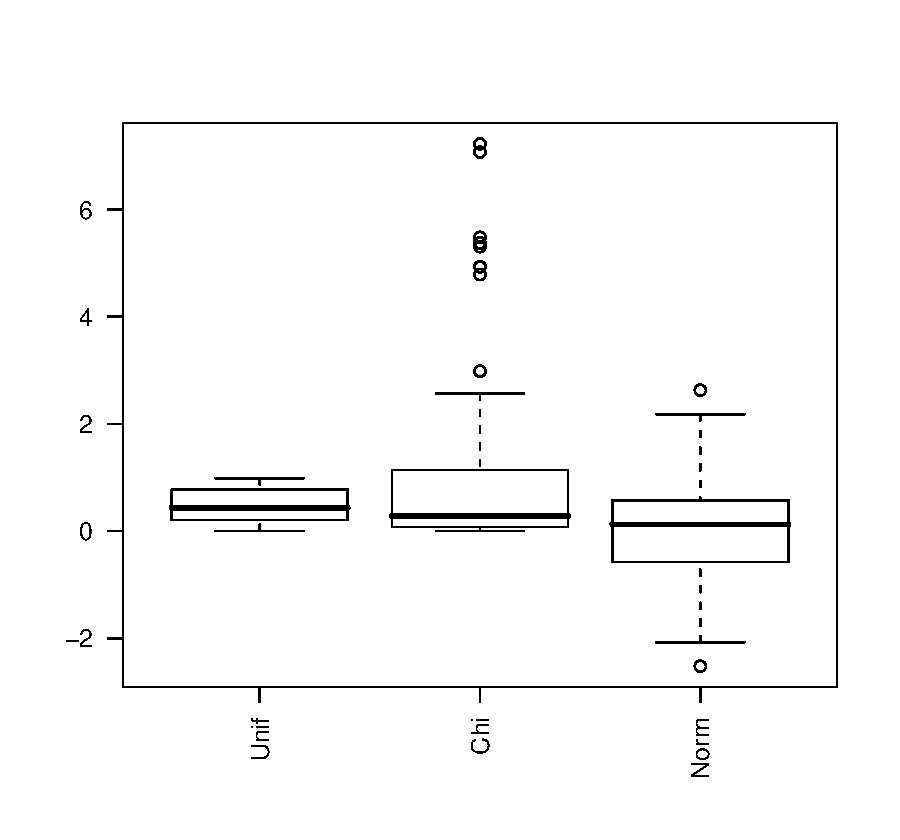
\includegraphics{plots/random-009}
  \end{centering} 
  \end{figure}
\end{frame}
 
%%%%%%%%%%%%%%%%%%%%%%%%%%%%%%%%%%%%%%%%%%%%%%%%%%%%%%%%%%%%%%%%%%%%%%%%%%%

\end{document}

